\documentclass[review,12pt,authoryear]{elsarticle}

\usepackage{amsmath,amssymb,amsthm,mathtools}
\usepackage{booktabs,longtable,array,multirow}
\usepackage{graphicx}
\usepackage[hidelinks]{hyperref}
\usepackage{lineno}
\modulolinenumbers[5]

\theoremstyle{plain}
\newtheorem{proposition}{Proposition}
\newtheorem{corollary}[proposition]{Corollary}
\theoremstyle{definition}
\newtheorem{assumption}{Assumption}
\newtheorem{remark}{Remark}

\newcommand{\E}{\mathbb{E}}
\newcommand{\Var}{\operatorname{Var}}
\newcommand{\Cov}{\operatorname{Cov}}
\newcommand{\Corr}{\operatorname{Corr}}
\newcommand{\plim}{\operatorname*{plim}}
\newcommand{\one}{\mathbf{1}}

\journal{Borsa Istanbul Review}

\begin{document}

\begin{frontmatter}

\title{What Financial Statements Can and Cannot Reveal About Monetary
Transmission to Corporate Balance Sheets: Evidence from Vietnam and
T\"{u}rkiye}

%% Double anonymized review: author information is in the separate title page.

\begin{abstract}
A productive literature shows that firms holding floating-rate debt bear the
brunt of monetary tightening. It rests almost entirely on supervisory credit
registries that record contract-level repricing terms. Most emerging markets
have no such registry available to researchers; what they have is published
financial statements. We ask, formally and empirically, whether the accounting
record can substitute. We develop a measurement framework in which exposure is
estimated rather than observed, and derive four results: the
difference-in-differences estimand is attenuated by exactly the reliability
ratio of the exposure measure; that ratio is identified by the split-half
correlation of independently estimated exposures; feasible estimation of
firm-level repricing sensitivities requires a panel length that annual
accounting data does not deliver; and an inflation-accounting restatement whose
magnitude depends on asset vintage enters the estimating equation as an
exposure-by-post interaction that two-way fixed effects cannot absorb, while
ratios of two flows are invariant to it up to a common factor. We then take
these predictions to harmonised panels of 693 Vietnamese and 585 Turkish listed
non-financial firms over 2010--2025, exploiting a natural contrast in dose:
T\"{u}rkiye tightened from 9\% to 47.5\% while Vietnam tightened mildly and
reversed. The constructive findings are that a simple implied borrowing cost
recovers each central bank's policy path without being given it, and that
pass-through is large but incomplete, at roughly 35\%, while median interest
coverage halves. The cautionary findings match the theory point for point:
split-half reliabilities of $-0.219$ and $-0.080$ imply a reliability ratio
indistinguishable from zero, in-sample fit matches the derived null benchmark
of $k/(T-1)$ almost exactly, and no exposure gradient survives once
contaminated outcomes are removed and the pre-period is long enough to test
parallel trends. We conclude that the contractual object these designs require
is not recoverable from published statements, and set out what is.
\end{abstract}

\begin{keyword}
monetary transmission \sep corporate default \sep measurement error \sep
inflation accounting \sep emerging markets \sep financial statements
\MSC[2020] 62P20 \sep 91G40
\JEL E52 \sep G32 \sep M41 \sep C23
\end{keyword}

\end{frontmatter}

\linenumbers

\section{Introduction}
\label{sec:intro}

A firm that borrows at a floating rate feels a policy tightening within weeks.
A firm that borrowed long and fixed does not feel it until it refinances. This
asymmetry is simple, intuitive, and has become the organising principle of a
productive literature on how monetary policy reaches the corporate sector.
\citet{ippolito2018} identify a \emph{floating rate channel} in matched
loan-level records, showing that firms with unhedged floating-rate bank debt cut
investment and employment more sharply after tightening. \citet{sengul2026},
studying the June 2023 policy reversal in T\"{u}rkiye, apply a two-part Double
Machine Learning design to a large administrative dataset and find that while
the average effect is modest, sensitivity concentrates in firms with weak
internal risk ratings, low liquidity and high exposure shares, with exporters
and manufacturers relatively insulated.

What these studies share is not merely a question but an input: a credit
registry recording, loan by loan, whether the contract reprices. Such registries
exist in relatively few jurisdictions and are available to researchers in fewer
still. What almost every market does have is a body of audited, published
financial statements. The question this paper takes seriously---and, we argue,
the field has not asked carefully enough---is whether that accounting record can
stand in for the registry.

The stakes are practical. If statements suffice, the literature's geographic
reach expands by an order of magnitude. If they do not, then a body of work is
being built on designs that cannot deliver what they promise, and it is worth
establishing precisely where the failure occurs and what remains possible.

\subsection{Approach}

We proceed in two stages. Section~\ref{sec:framework} develops a measurement
framework in which the exposure variable is \emph{estimated} rather than
observed, and derives what that implies for the difference-in-differences
estimand. The framework delivers four propositions, each of which generates a
sharp, falsifiable prediction about statistics we can compute. Sections
\ref{sec:setting}--\ref{sec:robust} take those predictions to data.

The empirical design is comparative. Vietnam and T\"{u}rkiye share the
structural features that make the floating-rate channel plausible:
bank-dominated corporate finance, thin corporate bond markets, heavy reliance on
short-maturity credit, and substantial listed non-financial sectors. What they
do not share is the monetary experience of 2021--2025. T\"{u}rkiye executed one
of the decade's most severe tightenings, from 9.0\% to 47.5\%, under inflation
exceeding 60\%. Vietnam tightened modestly in late 2022 and reversed within a
year.

This contrast is the paper's instrument. It supplies a strong dose and a weak
one, and it imposes a discipline single-country studies cannot: a measurement
strategy that works should register both, in proportion. A method reporting
similar magnitudes in both, or registering Vietnam more strongly than
T\"{u}rkiye, has failed a test it would never have faced alone.

Our diagnostic standard throughout is \emph{validation against an external
benchmark}. We do not ask whether a measure is statistically well behaved; we
ask whether it recovers something independently known. For the price of debt,
the benchmark is the published policy path. For exposure, it is the firm's own
subsequent change in borrowing cost. For the panel, it is an independent
commercial rendering of the same filings.

\subsection{What we find}

The constructive half of the answer concerns the \emph{price} of corporate debt.
A firm's implied borrowing cost---interest expense divided by average
debt---aggregates to a series reproducing each central bank's policy path
without being shown it. The Turkish series peaks in 2024, the year policy peaks;
the Vietnamese series traces the 2011 inflation crisis, the long easing through
2015, and the 2023 tightening. This establishes that ordinary filings carry a
legible signal of monetary transmission.

Two results follow. We quantify pass-through: a 38.5 percentage point Turkish
policy move produces a 13.4 point move in realised borrowing costs, roughly
35\%, while median interest coverage halves from 3.36 to 1.66.
Section~\ref{sec:framework} shows how to read that number structurally as an
effective repricing share. Second, the same diagnostic exposes a data hazard: a
widely used Turkish vendor field labelled \emph{Financial Expenses} bundles
foreign-exchange revaluation with interest, running roughly three times the true
figure, so measures built on it peak in the lira crises of 2018 and 2021 rather
than at the 2024 policy peak.

The cautionary half concerns \emph{exposure}, and here theory and evidence
coincide exactly. Proposition~\ref{prop:atten} shows that using an estimated
exposure attenuates the estimand by the reliability ratio $\lambda$.
Proposition~\ref{prop:split} shows $\lambda$ is identified by the split-half
correlation of independently estimated exposures. We measure that correlation at
$-0.219$ in T\"{u}rkiye and $-0.080$ in Vietnam, implying
$\hat{\lambda}\approx 0$: the estimand is attenuated to zero regardless of the
true effect, and a null is therefore uninformative about the underlying
parameter. Proposition~\ref{prop:feas} derives the panel length required for
feasible estimation and shows annual accounting data falls short by roughly an
order of magnitude. Proposition~\ref{prop:r2} derives the in-sample fit expected
under the null, $k/(T-1)\approx0.40$, against an observed Vietnamese median of
$0.396$.

Layered on top is a problem specific to high-inflation settings.
Proposition~\ref{prop:restate} shows that when non-monetary assets are restated
by a vintage-dependent factor while monetary debt is not, the distortion enters
as an exposure-by-post interaction that two-way fixed effects cannot absorb.
Proposition~\ref{prop:flow} shows that ratios of two flows escape it. We
demonstrate the former empirically: a standard specification returns highly
significant wrong-signed coefficients on a monotonically growing post-treatment
path.

\subsection{Why a null of this kind is informative}

Null results invite the suspicion of low power, and we address it directly.
Over the analysis three separate significant results appeared and each was shown
to be an artefact: a Turkish effect of $+0.886$ ($p=0.045$) that vanished when
the sample doubled; the FX results, which were accounting restatement; and the
final flow-based coefficients, which were pre-existing trend. Each was caught by
a diagnostic---sample expansion, an accounting-mechanics argument, an extended
event window---that a conventional specification would not have run. A design
generating three false positives before generating a null is informative about
the design.

\subsection{Contribution}

To the transmission literature we delimit where statement-based designs can
substitute for registry data, and supply a validated price measure that
survives. To empirical work on T\"{u}rkiye we document two hazards---one in a
vendor field, one in the accounting standard---threatening a broad class of
post-2022 studies. To research on Vietnam we introduce a firm-level statement
panel not previously used for such questions. Methodologically, we offer
split-half reliability and first-stage prediction as cheap, decisive tests that
any paper using an estimated firm characteristic as a regressor should report,
and we give them a formal justification.

\section{Related literature}
\label{sec:lit}

\subsection{Firm heterogeneity in monetary transmission}

That monetary policy affects firms unequally is long established.
\citet{gertler1994} documented that small manufacturing firms bear a
disproportionate share of the adjustment following tightening, and
\citet{bernanke1995} formalised the credit channel through which balance-sheet
strength mediates the response. \citet{kashyap2000} established the bank lending
channel using cross-sectional variation in bank liquidity.

The modern literature has sharpened the relevant margin. \citet{ottonello2020}
show that firms with low default risk respond \emph{most} to monetary shocks,
because they face flatter marginal cost curves for external finance.
\citet{cloyne2023} find that younger firms without dividend payments drive the
investment response. \citet{ozdagli2017} shows that financial frictions shape
the stock price reaction to policy, and \citet{greenwald2019} identifies an
interest coverage channel operating through debt covenants---directly relevant
to our outcome set, since coverage is one of the few distress measures that
survives Proposition~\ref{prop:flow}.

Two strands bear closely on our design. The first concerns \emph{contractual}
repricing: \citet{ippolito2018} identify the floating rate channel using
loan-level data, and \citet{auer2019} trace international transmission through
banks in small open economies. The second concerns \emph{maturity}:
\citet{almeida2012} exploit quasi-random variation in whether long-term debt
happened to mature just before the 2007 crisis, a design that isolates rollover
exposure cleanly; \citet{jungherr2024} show maturity structure materially shapes
transmission; \citet{hexiong2012} provide the theoretical link between rollover
and credit risk; and \citet{demirguc1999} document how institutions shape
maturity choice across countries.

Our contribution is not to this literature's substance but to its
transportability. Every study cited uses either supervisory data or a market
with rich contractual disclosure. We ask what remains when neither is available,
and Section~\ref{sec:framework} shows the answer is not simply ``a noisier
version of the same design''.

\subsection{Currency mismatch in emerging markets}

Because T\"{u}rkiye's episode combines tightening with severe depreciation, the
FX-mismatch literature bears directly on our measurement problem.
\citet{eichengreen1999} framed the ``original sin'' of borrowing in foreign
currency. The empirical record is more nuanced than the framing suggests:
\citet{bleakley2008} find that firms holding dollar debt did not systematically
underperform during depreciations, because they tended to hold dollar revenues
too, while \citet{aguiar2005} documents contractionary balance-sheet effects in
Mexico. \citet{kalemli2016} reconcile these by showing that the damaging
combination is unhedged FX debt together with a banking crisis restricting
credit supply.

\citet{bruno2015a,bruno2015b} establish the risk-taking channel linking exchange
rates, bank leverage and global liquidity; \citet{du2022} connect sovereign
risk, currency risk and corporate balance sheets; \citet{acharya2024} show how
impaired credit allocation distorts inflation dynamics. For T\"{u}rkiye,
\citet{akbal2026} examine the asymmetric response of the lira to capital flows
and sovereign spreads.

This literature matters to us twice over. Substantively it explains why
exporters may be insulated---a mechanism \citet{sengul2026} invoke directly,
noting that exporters generate foreign-currency revenues and benefit from
exchange-rate pass-through. Methodologically it explains why the bundled
financial-expense field of Section~\ref{sec:price} is so damaging: in a currency
crisis revaluation losses dwarf interest, and a measure conflating them
attributes currency effects to monetary policy.

\subsection{Accounting measurement under inflation}

Our identification problem is at bottom an accounting one, and there is a
literature on it that monetary economics rarely cites. \citet{gordon2001}
examines the value relevance of historical cost, price level and replacement
cost accounting in Mexico; \citet{barniv1999} studies inflation-adjusted versus
historical-cost earnings under hyperinflation; \citet{davisfriday2005} analyse
how the valuation roles of book value, earnings and cash flows shift during a
macroeconomic shock; and \citet{konchitchki2011} demonstrates that nominal
reporting has real consequences even at moderate inflation.
\citet{defranco2011} show that statement comparability is itself economically
consequential.

The consistent message is that when general price levels move sharply, the
mapping from economic reality to reported figures changes, and changes
\emph{differently across firms}. Proposition~\ref{prop:restate} gives this
literature what we believe is a novel application: an accounting transition
coinciding with a treatment date and interacting with the treatment variable is
not a nuisance to be absorbed but a threat to identification.

\subsection{Measurement error and generated regressors}

Our exposure results connect to a developed econometric literature.
\citet{pagan1984} established the consequences of using a regression-generated
variable as a regressor in a second stage, which is precisely our situation.
\citet{griliches1986} show that panel transformations frequently \emph{amplify}
rather than attenuate measurement error---directly relevant, since
first-differencing in \eqref{eq:beta} removes the fixed effect but magnifies the
noise-to-signal ratio. Classical attenuation biases coefficients toward zero,
exactly the pattern our null exhibits, which is why we regard a first-stage
validity test as obligatory rather than optional.

Proposition~\ref{prop:decomp} extends this in a direction we have not seen
applied to firm-level exposure: separating estimation error from genuine
impermanence of the underlying characteristic. The distinction is consequential
because the two failure modes call for opposite responses.

\section{A framework for statement-based exposure measurement}
\label{sec:framework}

This section formalises what is at stake when the exposure variable of a
difference-in-differences design is estimated from accounting data rather than
observed contractually. The framework is deliberately spare, and each result
generates a statistic we compute in Sections~\ref{sec:price}--\ref{sec:ident}.

\subsection{Setup}

Index firms by $i=1,\dots,N$ and years by $t=1,\dots,T$. Let $\pi_t$ denote the
policy rate and $f_t$ the log exchange rate. Let $P_t=\one\{t\ge t^{*}\}$ be the
post-treatment indicator, with $t^{*}$ the tightening date.

Each firm has a latent \emph{repricing exposure} $\theta_i$, defined as the
share of its debt whose contractual rate resets within the period. The object of
interest is the effect of tightening on a distress outcome $Y_{it}$, mediated by
exposure:
\begin{equation}
Y_{it} \;=\; \beta\,\bigl(\theta_i P_t\bigr) \;+\; \alpha_i \;+\; \lambda_t
\;+\; \varepsilon_{it},
\qquad \E[\varepsilon_{it}\mid \theta_i, P_t]=0,
\label{eq:structural}
\end{equation}
with firm effects $\alpha_i$ and year effects $\lambda_t$. If $\theta_i$ were
observed, $\beta$ would be identified by the two-way within estimator. The
registry literature is, in effect, the case in which $\theta_i$ is observed.

Our situation is that $\theta_i$ is not disclosed. We observe instead a proxy
\begin{equation}
\widehat{\theta}_i \;=\; \theta_i + u_i,
\qquad u_i \perp (\theta_i,\varepsilon_{it}),
\qquad \Var(u_i)=\sigma_u^2,\ \ \Var(\theta_i)=\sigma_\theta^2 .
\label{eq:proxy}
\end{equation}
Define the \emph{reliability ratio}
\begin{equation}
\lambda \;\equiv\; \frac{\sigma_\theta^2}{\sigma_\theta^2+\sigma_u^2}\ \in[0,1].
\label{eq:lambda}
\end{equation}

\subsection{Attenuation of the treatment estimand}

\begin{proposition}[Attenuation]
\label{prop:atten}
Let $\widehat{\beta}$ be the two-way within estimator of \eqref{eq:structural}
obtained by replacing $\theta_i$ with $\widehat{\theta}_i$. Then
\begin{equation}
\plim_{N\to\infty}\ \widehat{\beta} \;=\; \lambda\,\beta .
\end{equation}
\end{proposition}

\begin{proof}
Write the regressor as $X_{it}=\widehat{\theta}_iP_t$ and let $\tilde{X}$ denote
its residual after projecting out firm and year effects. Because $P_t$ varies
only over time and $\widehat{\theta}_i$ only across firms, the within
transformation yields
$\tilde{X}_{it}=(\widehat{\theta}_i-\bar{\theta})(P_t-\bar{P})$. Using
\eqref{eq:proxy} and $u_i\perp\theta_i$,
\[
\Cov(\tilde{Y},\tilde{X})=\beta\,\sigma_\theta^2\,\Var(P),
\qquad
\Var(\tilde{X})=(\sigma_\theta^2+\sigma_u^2)\,\Var(P).
\]
The ratio is $\lambda\beta$. \end{proof}

Proposition~\ref{prop:atten} is the classical attenuation result
\citep{pagan1984} transposed to an interaction term, and it has an
uncomfortable implication: a statistically insignificant $\widehat{\beta}$ is
consistent with \emph{any} value of $\beta$ once $\lambda$ is small. A null is
therefore uninterpretable without an estimate of $\lambda$.

\subsection{Identifying the reliability ratio}

The natural objection is that $\lambda$ is unobservable because $\theta_i$ is.
It is not, provided two independent proxies can be constructed.

\begin{proposition}[Split-half identification]
\label{prop:split}
Let $\widehat{\theta}^{(1)}_i=\theta_i+u^{(1)}_i$ and
$\widehat{\theta}^{(2)}_i=\theta_i+u^{(2)}_i$ be estimated on disjoint
subsamples, with $u^{(1)}\perp u^{(2)}$ and
$\Var(u^{(1)})=\Var(u^{(2)})=\sigma^2_u$. Then
\begin{equation}
\Corr\bigl(\widehat{\theta}^{(1)},\widehat{\theta}^{(2)}\bigr)
\;=\;\frac{\sigma_\theta^2}{\sigma_\theta^2+\sigma_u^2}\;=\;\lambda .
\end{equation}
\end{proposition}

\begin{proof}
$\Cov(\widehat{\theta}^{(1)},\widehat{\theta}^{(2)})
=\Var(\theta)=\sigma_\theta^2$ since the errors are mutually independent and
independent of $\theta$. Each variance is $\sigma_\theta^2+\sigma_u^2$.
\end{proof}

\begin{corollary}
\label{cor:uninformative}
If the split-half correlation is not bounded away from zero, then
$\plim\widehat{\beta}=0$ irrespective of $\beta$, and the estimated treatment
effect carries no information about the structural parameter.
\end{corollary}

This is, to our knowledge, an underused device. The split-half correlation is
trivial to compute whenever exposure is estimated from a time series, and by
Proposition~\ref{prop:split} it \emph{is} the attenuation factor rather than
merely a diagnostic correlated with it. Section~\ref{sec:exposure} reports
values of $-0.219$ and $-0.080$.

\subsection{Feasibility: how long a panel is required?}

Corollary~\ref{cor:uninformative} raises the question of whether a longer panel
would rescue the design. It can be answered analytically.

Suppose exposure is estimated firm by firm from the first-differenced
regression
\begin{equation}
\Delta r_{it} \;=\; a_i \;+\; \theta_i\,\Delta\pi_t \;+\; \gamma_i\,\Delta f_t
\;+\; \eta_{it},
\qquad \Var(\eta_{it})=\sigma^2_\eta ,
\label{eq:beta}
\end{equation}
where $r_{it}$ is the firm's realised borrowing cost. With $T$ usable
observations per firm, sample variance $s^2_\pi$ of $\Delta\pi_t$, and
correlation $\rho$ between $\Delta\pi_t$ and $\Delta f_t$, the sampling variance
of the OLS estimate is
\begin{equation}
\Var(\widehat{\theta}_i)\;=\;\frac{\sigma^2_\eta}{T\,s^2_\pi\,(1-\rho^2)}
\;\equiv\;\sigma^2_u .
\label{eq:sampvar}
\end{equation}

\begin{proposition}[Feasibility condition]
\label{prop:feas}
Attaining reliability $\lambda\ge\lambda^{*}$ requires
\begin{equation}
T \;\ge\; \frac{\lambda^{*}}{1-\lambda^{*}}\,
\cdot\,\frac{\sigma^2_\eta}{s^2_\pi\,(1-\rho^2)\,\sigma^2_\theta}.
\label{eq:feas}
\end{equation}
\end{proposition}

\begin{proof}
Substitute \eqref{eq:sampvar} into \eqref{eq:lambda} and solve the inequality
$\sigma^2_\theta/(\sigma^2_\theta+\sigma^2_u)\ge\lambda^{*}$ for $T$.
\end{proof}

Every quantity on the right is estimable, so \eqref{eq:feas} can be taken to
data. When we do so in Section~\ref{sec:exposure} the condition is comfortably
satisfied: sampling noise implies $\lambda\approx0.99$ in Vietnam and $0.78$ in
T\"{u}rkiye, and a conventional power calculation would have judged the design
feasible at the available panel length.

That verdict is contradicted by the split-half correlations, which are zero or
negative. The contradiction is informative, and resolving it requires enriching
\eqref{eq:proxy}.

\subsection{Permanent, transitory and sampling components}

Suppose the quantity a firm-level regression recovers is not a fixed trait but a
window-specific realisation,
\begin{equation}
\theta_{i}^{(w)} \;=\; \theta_i \;+\; \nu_i^{(w)},
\qquad \Var(\nu^{(w)}_i)=\sigma^2_\nu,
\label{eq:transitory}
\end{equation}
where $\theta_i$ is a persistent characteristic and $\nu^{(w)}_i$ a transitory
component that is real within window $w$---the firm genuinely did reprice that
way over those years---but does not carry across windows. The estimated slope is
then $\widehat{\theta}^{(w)}_i=\theta_i+\nu^{(w)}_i+u^{(w)}_i$.

\begin{proposition}[Three-way decomposition]
\label{prop:decomp}
Under \eqref{eq:transitory} with $\nu$, $u$ mutually independent and
independent of $\theta$,
\begin{equation}
\Var(\widehat{\theta}^{(w)}_i)=\sigma^2_\theta+\sigma^2_\nu+\sigma^2_u,
\qquad
\Corr\bigl(\widehat{\theta}^{(1)},\widehat{\theta}^{(2)}\bigr)
=\frac{\sigma^2_\theta}{\sigma^2_\theta+\sigma^2_\nu+\sigma^2_u},
\end{equation}
so the split-half correlation identifies the \emph{permanent} share alone, and
\begin{equation}
\sigma^2_\nu \;=\; \Var(\widehat{\theta})\bigl(1-\Corr\bigr)\;-\;\sigma^2_u .
\end{equation}
Moreover, Proposition~\ref{prop:atten} continues to hold with $\lambda$ equal to
this permanent share, since only $\theta_i$ is stable enough to interact with a
treatment occurring after the estimation window.
\end{proposition}

\begin{proof}
The variance decomposition is immediate from independence. The covariance across
windows is $\Var(\theta)=\sigma^2_\theta$ because both $\nu$ and $u$ are
window-specific. Rearranging gives $\sigma^2_\nu$. \end{proof}

Proposition~\ref{prop:decomp} separates two failure modes that are easily
conflated. \emph{Imprecision} ($\sigma^2_u$ large) is remediable by more data.
\emph{Impermanence} ($\sigma^2_\nu$ large) is not: no amount of additional data
makes a transitory quantity a usable pre-determined regressor. The empirical
decomposition in Section~\ref{sec:exposure} attributes 99.4\% of Vietnamese and
78.0\% of Turkish dispersion in estimated slopes to the transitory component and
none to the permanent one---so the binding problem is impermanence, and
quarterly estimation would not solve it.

\subsection{In-sample fit is not evidence}

A researcher inspecting \eqref{eq:beta} would observe a respectable $R^2$ and
might conclude the specification has content. It does not.

\begin{proposition}[Null benchmark for fit]
\label{prop:r2}
Under the null that neither regressor enters \eqref{eq:beta}, with $k$
regressors excluding the intercept and $T$ observations, the coefficient of
determination satisfies
\begin{equation}
R^2 \sim \mathrm{Beta}\!\left(\tfrac{k}{2},\ \tfrac{T-k-1}{2}\right),
\qquad
\E\bigl[R^2\bigr] \;=\; \frac{k}{T-1}.
\end{equation}
\end{proposition}

\begin{proof}
Standard: under the null the explained and residual sums of squares are
independent $\chi^2$ variates with $k$ and $T-k-1$ degrees of freedom, so their
normalised ratio is Beta distributed with the stated parameters, whose mean is
$k/(T-1)$. \end{proof}

With $k=2$ and a median of $T=6$ usable observations, $\E[R^2]=0.40$. Any
reported fit near this value is uninformative. Section~\ref{sec:exposure}
reports an observed Vietnamese median of $0.396$.

\subsection{Inflation restatement as an exposure-by-post confound}

We now formalise the accounting problem described in
Section~\ref{sec:setting}. Let $A_{it}$ denote true non-monetary assets and
$D_{it}$ monetary debt. Under a general price-level restatement beginning at
$t_0$, non-monetary items are indexed by a factor depending on their
\emph{vintage}, while monetary items are not:
\begin{equation}
A^{*}_{it} \;=\; \Phi_{it}\,A_{it},
\qquad
D^{*}_{it} \;=\; D_{it},
\qquad
\log\Phi_{it} \;=\; \bigl(1+\delta_i\bigr)\,c_t\,\one\{t\ge t_0\},
\label{eq:restate}
\end{equation}
where $c_t$ is the common cumulative price-index component and $\delta_i$ is a
firm-specific loading determined by the vintage profile of the firm's asset
base, normalised so that $\E[\delta_i]=0$.

\begin{proposition}[Non-absorbability]
\label{prop:restate}
Let reported log leverage be $\ell^{*}_{it}=\log D^{*}_{it}-\log A^{*}_{it}$ and
consider the two-way within regression of $\ell^{*}_{it}$ on
$\theta_i P_t$ with $P_t=\one\{t\ge t_0\}$. Then
\begin{equation}
\plim\ \widehat{\beta}
\;=\;\beta \;-\; \bar{c}\,\frac{\Cov(\theta_i,\delta_i)}{\Var(\theta_i)},
\qquad \bar{c}\equiv\E\bigl[c_t\mid t\ge t_0\bigr],
\end{equation}
so the estimator is inconsistent whenever $\Cov(\theta_i,\delta_i)\neq0$, and
the bias is not removed by firm or year effects.
\end{proposition}

\begin{proof}
Substituting \eqref{eq:restate},
$\ell^{*}_{it}=\ell_{it}-c_t\one\{t\ge t_0\}-\delta_i c_t\one\{t\ge t_0\}$. The
second term varies only with $t$ and is absorbed by $\lambda_t$. The third term
varies across firms and only after $t_0$; it is therefore collinear with the
regressor $\theta_iP_t$ to the extent that $\delta_i$ covaries with $\theta_i$,
and projecting it onto $\theta_iP_t$ yields the stated bias. Firm effects
$\alpha_i$ cannot absorb it because it is zero before $t_0$ and non-zero after.
\end{proof}

Proposition~\ref{prop:restate} is the paper's central identification result and
the reason we regard the Turkish post-2022 window as hazardous. The condition
$\Cov(\theta_i,\delta_i)\neq0$ is not a knife-edge case: $\delta_i$ depends on
asset vintage, which correlates with capital intensity, sector and firm age,
each of which correlates with financing structure and hence with any
balance-sheet exposure measure. The usual defence---country-by-year fixed
effects---absorbs $c_t$ exactly and $\delta_ic_t$ not at all.

\subsection{Flow ratios are invariant}

The corresponding positive result identifies what survives.

\begin{proposition}[Flow invariance]
\label{prop:flow}
Suppose income-statement items accruing within period $t$ are restated by a
common factor $\psi_t$ that does not depend on $i$. Then for any two flows
$X_{it},Z_{it}$ the reported ratio is exactly invariant,
$X^{*}_{it}/Z^{*}_{it}=X_{it}/Z_{it}$; and for the implied borrowing cost
$r_{it}=|\mathrm{Int}_{it}|/\bar{D}_{it}$, which divides a restated flow by an
unrestated monetary stock,
\begin{equation}
\log r^{*}_{it} \;=\; \log\psi_t \;+\; \log r_{it},
\end{equation}
so that $\log r^{*}_{it}$ is contaminated only by an additive time effect, fully
absorbed by $\lambda_t$.
\end{proposition}

\begin{proof}
Immediate from $X^{*}=\psi_tX$, $Z^{*}=\psi_tZ$ and $D^{*}=D$. \end{proof}

\begin{remark}
Proposition~\ref{prop:flow} is why our outcome set is restricted to the EBIT
margin, interest coverage, the log implied rate and log debt growth, and why the
Altman $Z''$ score, leverage, equity ratios and return on assets are discarded:
each of the latter contains a non-monetary stock and is exposed to
Proposition~\ref{prop:restate}. It also refines the specification: the implied
rate is invariant \emph{in logs}, not in levels, and we use it accordingly.
\end{remark}

\subsection{Reading pass-through structurally}

Finally, the framework gives the aggregate pass-through estimate an
interpretation. Let the firm's realised average cost be a maturity-weighted
average of past marginal rates,
\begin{equation}
r_{it} \;=\; \sum_{s\ge0}\omega_{is}\,\iota_{t-s},
\qquad \sum_{s\ge0}\omega_{is}=1,
\end{equation}
where $\iota_t$ is the marginal contract rate and $\omega_{is}$ the share of
debt priced $s$ periods ago. Then $\partial r_{it}/\partial\iota_t=\omega_{i0}
\equiv m_i$, the share repricing within the period, and aggregating,
$\Delta\bar{r}/\Delta\bar{\iota}=\bar{m}$.

\begin{corollary}
\label{cor:passthrough}
The aggregate pass-through coefficient identifies the mean effective repricing
share $\bar{m}$ of the corporate debt stock.
\end{corollary}

Section~\ref{sec:price} estimates $\bar{m}\approx0.35$ for T\"{u}rkiye against a
median short-term debt share of $0.63$, implying that even nominally short debt
repriced only partially---evidence, though not proof, of quantity rationing or
subsidised credit substituting for full price adjustment.

\section{Institutional setting}
\label{sec:setting}

\subsection{Two monetary regimes}

The Turkish tightening is the sharper of the two by an order of magnitude.
After a period of unorthodox easing the one-week repo rate stood at 9.0\% at
end-2022. Following the June 2023 reversal it reached 42.5\% by end-2023, peaked
at 47.5\% during 2024, and stood at 38.0\% at end-2025. Consumer price inflation
exceeded 60\% at its height and the lira depreciated from roughly 18.7 per US
dollar at end-2022 to 43.0 at end-2025.

Vietnam's experience is far milder. The State Bank raised policy rates in late
2022 amid stress in the domestic corporate bond market and reversed through
2023. The average bank lending rate rose from 8.0\% in 2022 to 9.3\% in
2023---against 17.0\% at the peak of the 2011 inflation episode, a useful
within-country benchmark for what a severe Vietnamese tightening looks like.

The comparison is therefore not treatment versus control but large dose versus
small dose, and the appropriate prediction is proportional rather than binary.

\subsection{The Turkish accounting transition}

T\"{u}rkiye met the IFRS criteria for a hyperinflationary economy and was
classified as such from April 2022, with local inflation-adjustment
requirements following for statements through end-2023. Under the relevant
standard, entities reporting in the currency of a hyperinflationary economy
restate their statements in the measuring unit current at the balance sheet
date, and comparatives are restated on the same basis.

The mechanics are those assumed in \eqref{eq:restate}. Non-monetary
items---property, plant and equipment, inventories, equity---are restated by a
general price index applied from each item's acquisition date, so the effective
factor depends on vintage. Monetary items---debt, cash, receivables---are
already in period-end purchasing power and are not restated. Income-statement
items are restated to period-end purchasing power by a factor common across
firms within a period, which is the condition of Proposition~\ref{prop:flow}.

\section{Data}
\label{sec:data}

\subsection{Sources and construction}

The Vietnamese panel derives from an item-level dataset of statements filed by
companies listed on the Ho Chi Minh City and Hanoi exchanges, distributed
through a public research repository in long format with standardised item
codes. Pivoting to firm-year observations yields 9{,}893 firm-years for 693
firms over 2011--2025, with non-missing coverage of 94.5\% for total assets,
94.7\% for total debt, 91.2\% for interest expense, 93.2\% for EBIT and 96.8\%
for equity.

The Turkish panel derives from a brokerage service redistributing filings made
to the Public Disclosure Platform. One request returns the balance sheet, income
statement, cash-flow statement and supplementary items with bilingual labels for
four annual periods. The resulting panel covers 585 firms over 2010--2025 and
carries two items with no Vietnamese counterpart: export sales and net
foreign-currency position.

Both panels are restricted to non-financial firms, since banks, insurers and
brokers file on incompatible templates. We require strictly positive total debt
and assets, the transmission channel being undefined otherwise.

\begin{table}[htbp]
\centering
\caption{Firms per year}
\label{tab:coverage}
\begin{tabular}{lrr@{\hskip 2em}lrr}
\toprule
Year & T\"{u}rkiye & Vietnam & Year & T\"{u}rkiye & Vietnam \\
\midrule
2015 & 349 & 648 & 2021 & 551 & 691 \\
2016 & 358 & 663 & 2022 & 568 & 692 \\
2017 & 370 & 670 & 2023 & 585 & 693 \\
2018 & 428 & 682 & 2024 & 584 & 692 \\
2019 & 467 & 686 & 2025 & 582 & 689 \\
2020 & 508 & 690 &      &     &     \\
\bottomrule
\end{tabular}
\end{table}

\subsection{Descriptive statistics}

\begin{table}[htbp]
\centering
\caption{Descriptive statistics, 2015--2025}
\label{tab:desc}
\begin{tabular}{lrrrr@{\hskip 1.5em}rrrr}
\toprule
& \multicolumn{4}{c}{Vietnam} & \multicolumn{4}{c}{T\"{u}rkiye} \\
\cmidrule(lr){2-5}\cmidrule(lr){6-9}
Variable & $n$ & Mean & Median & SD & $n$ & Mean & Median & SD \\
\midrule
Debt / assets            & 5{,}708 & 0.250 & 0.225 & 0.170 & 4{,}780 & 0.228 & 0.195 & 0.190 \\
Short-term debt share    & 5{,}708 & 0.709 & 0.852 & 0.323 & 4{,}783 & 0.627 & 0.647 & 0.284 \\
Implied borrowing cost   & 5{,}693 & 0.063 & 0.063 & 0.032 & 3{,}870 & 0.312 & 0.252 & 0.219 \\
Interest coverage        & 5{,}340 & 9.225 & 3.290 & 15.698 & 4{,}673 & 2.680 & 1.068 & 6.502 \\
Return on assets         & 5{,}698 & 0.065 & 0.053 & 0.065 & 4{,}783 & 0.080 & 0.070 & 0.105 \\
\bottomrule
\end{tabular}
\end{table}

Leverage is comparable across markets at 20--25\% of assets, and both corporate
sectors fund themselves predominantly at short maturity; the Vietnamese median
short-term share of 0.85 speaks to the rollover-risk framing of
\citet{hexiong2012}. The contrast in distress is stark: median Turkish interest
coverage is 1.07 against Vietnam's 3.29, placing the median Turkish firm close
to the covenant-relevant threshold \citet{greenwald2019} identifies.

\subsection{Cross-validation against an independent source}

Because the subject is measurement, we test rather than assume our panels.

\begin{table}[htbp]
\centering
\caption{Reconciliation with an independent source}
\label{tab:xval}
\begin{tabular}{lrrrr}
\toprule
& \multicolumn{2}{c}{Vietnam} & \multicolumn{2}{c}{T\"{u}rkiye} \\
\cmidrule(lr){2-3}\cmidrule(lr){4-5}
Variable & Corr. & Median diff. & Corr. & Median diff. \\
\midrule
Total assets              & 1.0000 & 0.0000 & 0.9960 & 0.0000 \\
Revenue                   & 0.9999 & 0.0000 & 0.9935 & 0.0000 \\
Total debt                & 0.9906 & 0.0000 & 0.9960 & $-0.0295$ \\
Equity                    & 0.9956 & $-0.0447$ & 0.9552 & $-0.0039$ \\
EBIT                      & 0.7657 & $+0.2339$ & 0.8539 & $+0.2093$ \\
Interest expense (abs.)   & 0.9913 & 0.0000 & \textbf{0.7272} & $\mathbf{-0.6880}$ \\
\bottomrule
\end{tabular}
\end{table}

Total assets and revenue reconcile at a median relative difference of zero in
both countries. Equity differs by about four percent in Vietnam because the
aggregator reports parent-only equity where the national source consolidates
minority interest; EBIT differs by 21--23\% because the aggregator derives it
from pretax income plus interest rather than reported operating profit. Both are
definitional. The interest-expense discrepancy in T\"{u}rkiye is not, and
Section~\ref{sec:price} is devoted to it.

\section{The price of corporate debt}
\label{sec:price}

\subsection{Construction and validation}

For firm $i$ in year $t$ the implied borrowing cost is
\begin{equation}
r_{it} \;=\; \frac{|\mathrm{Interest\ expense}_{it}|}
{\tfrac{1}{2}\bigl(D_{it}+D_{i,t-1}\bigr)} ,
\label{eq:impliedrate}
\end{equation}
with $D$ the sum of short- and long-term borrowings. Averaging the denominator
prevents the ratio being driven mechanically by borrowing undertaken during the
year. By Proposition~\ref{prop:flow}, $\log r_{it}$ is contaminated only by an
additive time effect under restatement, and we use logs throughout.

The measure is not calibrated to any policy series, so recovering one is a
genuine test.

\begin{table}[htbp]
\centering
\caption{Median implied borrowing cost and the policy path}
\label{tab:validate}
\begin{tabular}{lrr@{\hskip 2em}lrr}
\toprule
\multicolumn{3}{c}{Vietnam} & \multicolumn{3}{c}{T\"{u}rkiye} \\
\cmidrule(lr){1-3}\cmidrule(lr){4-6}
Year & Implied & Lending rate & Year & Implied & CBRT policy \\
\midrule
2011 & 11.1\% & 17.0\% & 2022 & 17.8\% & 9.0\% \\
2013 & 7.5\%  & 10.4\% & 2023 & 25.4\% & 42.5\% \\
2015 & 5.8\%  & 7.1\%  & 2024 & \textbf{31.2\%} & \textbf{47.5\%} \\
2020 & 6.3\%  & 7.6\%  & 2025 & 25.8\% & 38.0\% \\
2023 & 7.2\%  & 9.3\%  &      &        &        \\
2025 & 5.8\%  & ---    &      &        &        \\
\bottomrule
\end{tabular}
\end{table}

\begin{figure}[htbp]
\centering
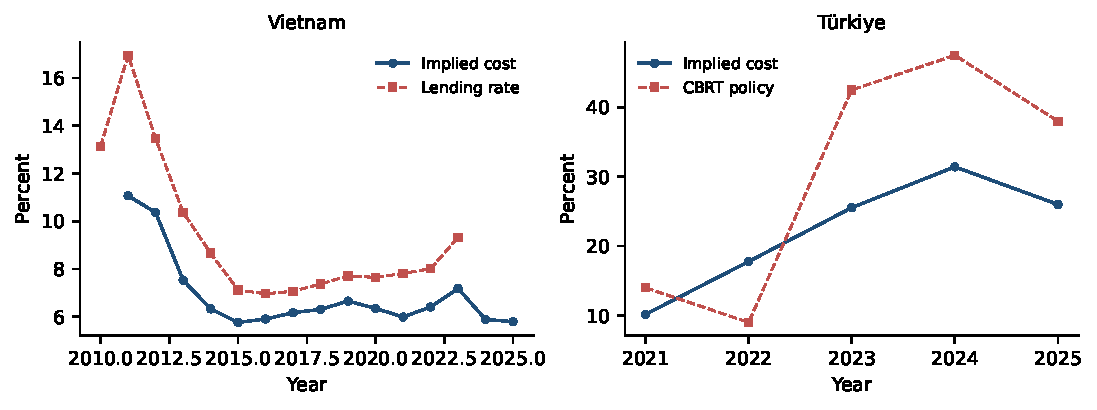
\includegraphics[width=\textwidth]{figs/validation.pdf}
\caption{Median implied borrowing cost against the policy path. The measure is
constructed from firm financial statements alone and is not calibrated to any
policy series.}
\label{fig:validation}
\end{figure}

Figure~\ref{fig:validation} plots the comparison. The Turkish series peaks in
2024, the year policy peaks. The Vietnamese series
peaks in 2011 at the height of that country's inflation crisis, falls
monotonically to 5.8\% by 2015, rises to 7.2\% in the 2023 tightening and
subsides. Median interest coverage moves in mirror image, reaching its
Vietnamese sample minimum of 2.05 in exactly 2023.

\subsection{Pass-through}

Policy moved 38.5 points between end-2022 and the 2024 Turkish peak; realised
borrowing costs moved 13.4 points, from 17.8\% to 31.2\%. By
Corollary~\ref{cor:passthrough} this identifies a mean effective repricing share
of $\bar{m}\approx0.35$. Set against a median short-term debt share of $0.63$,
it implies that even nominally short debt repriced only partially. Over the same
window median interest coverage halved, from 3.36 to 1.66. Vietnam's mild cycle
moves costs 0.8 points, with coverage dipping from 3.11 to 2.05 and recovering
to 2.70.

\subsection{A data hazard: bundled financial expense}

The Turkish field labelled \emph{Financial Expenses} is the only interest-like
item available before 2021 and is the natural candidate for the long history. It
should not be used as one: against the independent aggregator it runs roughly
three times larger, with a median relative difference of $-68.8\%$ and a
correlation of $0.727$ on absolute values, against Vietnam's $0.991$ and
$0.00\%$.

The field bundles foreign-exchange revaluation, and in a currency crisis those
losses dwarf interest. The consequence is not attenuation but a change in what
is measured: built on the bundled field the Turkish implied cost peaks in
\textbf{2018 and 2021}, the lira depreciation episodes; built on a clean
interest figure it peaks in \textbf{2024}, with policy. A researcher using it to
study monetary transmission would recover currency shocks and report them as
interest-rate effects, with strong significance.

\section{Measuring exposure}
\label{sec:exposure}

\subsection{The required object is not disclosed}

Contractual repricing basis does not appear in published statements under either
regime. Firms disclose borrowings by maturity and sometimes currency, but not by
repricing terms. We therefore assess the two constructible substitutes.

\subsection{Revealed repricing sensitivity}

We estimate \eqref{eq:beta} firm by firm over a window ending before treatment.
The FX term is included jointly rather than as a nuisance control, because
Section~\ref{sec:price} established that much of the movement in Turkish
realised cost is currency revaluation.

On conventional diagnostics the estimates behave: about 72\% of firms in both
countries return a positive $\widehat{\theta}$, the mean Vietnamese estimate
implies that a one-point rise in the lending rate raises a firm's cost of funds
by roughly 0.79 points, and median in-sample $R^2$ is 0.28 in Vietnam and 0.34
in T\"{u}rkiye. Propositions~\ref{prop:split}--\ref{prop:r2} supply the tests
these diagnostics cannot pass.

\begin{table}[htbp]
\centering
\caption{Split-half reliability of candidate exposure measures}
\label{tab:split}
\begin{tabular}{lrr}
\toprule
Measure & T\"{u}rkiye & Vietnam \\
\midrule
Repricing sensitivity $\widehat{\theta}$ & $\mathbf{-0.219}$ & $\mathbf{-0.080}$ \\
FX sensitivity $\widehat{\gamma}$        & $+0.147$ & $+0.094$ \\
Short-term debt share                    & $+0.438$ & $+0.628$ \\
Export share                             & $+0.838$ & --- \\
\bottomrule
\end{tabular}
\end{table}

By Proposition~\ref{prop:split} these correlations \emph{are} the reliability
ratio $\lambda$. Both are zero or negative, so by
Corollary~\ref{cor:uninformative} the treatment estimand is attenuated to zero
and carries no information about $\beta$. The measured balance-sheet
characteristics in the lower rows behave as stable traits, so the failure is
specific to regression-estimated quantities.

\begin{table}[htbp]
\centering
\caption{Variance decomposition of estimated repricing sensitivities}
\label{tab:decomp}
\begin{tabular}{lrr}
\toprule
& Vietnam & T\"{u}rkiye \\
\midrule
$\Var(\widehat{\theta})$                       & $3.75\times10^{-3}$ & $1.74\times10^{-4}$ \\
Sampling component $\sigma^2_u$                & $2.42\times10^{-5}$ & $3.83\times10^{-5}$ \\
Reliability implied by sampling noise alone    & 0.994 & 0.780 \\
Measured split-half correlation                & $-0.080$ & $-0.219$ \\
Permanent component $\sigma^2_\theta$          & 0.000 & 0.000 \\
Transitory component $\sigma^2_\nu$            & $3.73\times10^{-3}$ & $1.36\times10^{-4}$ \\
Transitory share of dispersion                 & \textbf{99.4\%} & \textbf{78.0\%} \\
\bottomrule
\end{tabular}
\end{table}

Table~\ref{tab:decomp} applies Proposition~\ref{prop:decomp} and delivers the
paper's sharpest methodological finding. Sampling noise alone implies
reliabilities of 0.994 and 0.780: a conventional power calculation, or an
inspection of standard errors, would have judged the design comfortably
feasible. The split-half correlations nonetheless force the permanent component
to zero, attributing 99.4\% of Vietnamese and 78.0\% of Turkish dispersion to a
transitory component.

The distinction matters for what one should do about it. Imprecision is
remediable with more data; impermanence is not. A firm's estimated repricing
sensitivity is real within the window in which it is measured and does not
persist beyond it, so it cannot serve as a pre-determined regressor for a
treatment occurring later. Quarterly estimation would raise $T$ and shrink
$\sigma^2_u$, which Table~\ref{tab:decomp} shows was never the binding
constraint.

\subsection{First-stage prediction}

The decisive test asks whether $\widehat{\theta}$ predicts what it purports to.

\begin{table}[htbp]
\centering
\caption{Does estimated exposure predict the actual change in borrowing cost?}
\label{tab:firststage}
\begin{tabular}{lrr}
\toprule
& T\"{u}rkiye (2022--24) & Vietnam (2022--23) \\
\midrule
Coefficient on $\widehat{\theta}$ (standardised) & $-0.036$ & $+0.001$ \\
$p$-value                                        & 0.27 & 0.54 \\
$R^2$                                            & 0.035 & 0.002 \\
Change, lowest tercile                           & $+0.19$ & $+0.006$ \\
Change, highest tercile                          & $\mathbf{+0.04}$ & $+0.010$ \\
\bottomrule
\end{tabular}
\end{table}

In T\"{u}rkiye the most-exposed tercile records the \emph{smallest} increase in
realised cost. Median in-sample fit of 0.396 in Vietnam matches the null
benchmark $k/(T-1)=0.40$ of Proposition~\ref{prop:r2} almost exactly.

\subsection{Balance-sheet proxies}

The measured characteristics are reliable but do not identify repricing.
Regressing the actual change in borrowing cost on standardised pre-period
characteristics yields $R^2$ below $0.02$ for the short-term debt share,
leverage, the current ratio, size and interest coverage, in both countries.

The short-maturity share illustrates the confound. It is simultaneously a
measure of repricing exposure and of credit quality, since firms able to roll
short-term paper cheaply are disproportionately the strongest borrowers. In
T\"{u}rkiye the two align and coverage falls monotonically across terciles; in
Vietnam the credit-quality effect dominates and the ordering inverts, the
most short-funded tercile being the healthiest in most years ($5.02$ against
$3.45$ in 2021). A proxy whose sign flips across two structurally similar
markets is not measuring a single construct.

\section{Identification}
\label{sec:ident}

\subsection{The restatement confound, empirically}

\begin{table}[htbp]
\centering
\caption{Turkish median balance-sheet aggregates}
\label{tab:restate}
\begin{tabular}{lrr}
\toprule
Year & Equity / assets & Debt / assets \\
\midrule
2017 & 0.472 & 0.217 \\
2019 & 0.419 & 0.226 \\
2021 & 0.462 & 0.189 \\
\textbf{2022} & \textbf{0.558} & \textbf{0.138} \\
\textbf{2023} & \textbf{0.614} & \textbf{0.111} \\
2024 & 0.646 & 0.100 \\
2025 & 0.619 & 0.117 \\
\bottomrule
\end{tabular}
\end{table}

Median leverage more than halves between 2019 and 2024 while equity-to-assets
rises by over twenty points, in a period of severe tightening and depreciation
during which no such deleveraging occurred. The break begins in 2022, consistent
with the April 2022 classification and the restatement of comparatives.

Proposition~\ref{prop:restate} predicts that a design using stock-based outcomes
will be inconsistent whenever $\Cov(\theta_i,\delta_i)\neq0$. Estimating it with
FX exposure as treatment returns exactly that pathology: coefficients that are
highly significant and wrongly signed, with firms holding more foreign-currency
debt appearing to \emph{improve} after 2023 (implied rate $-0.108$, $p<0.0001$;
Altman $Z''$ $+0.813$, $p=0.004$; leverage $-0.049$, $p<0.0001$); an event-study
path growing monotonically as restatement compounds ($+0.32$, $+0.83$, $+1.18$
across 2023--2025); and large significant pre-treatment coefficients. The result
has every outward mark of a strong causal finding and is an accounting artefact.

\subsection{The surviving specification}

Propositions~\ref{prop:restate} and \ref{prop:flow} imply three restrictions.
Outcomes must be flows: we retain the log implied rate, interest coverage, EBIT
margin and log debt growth, and discard the Altman $Z''$ score, leverage, equity
ratios and return on assets. Exposure must predate the restatement, and we
measure it at 2021. And the pre-period must permit a test of parallel trends;
because EBIT margin and debt growth require no interest figure, the bundling
problem of Section~\ref{sec:price} is irrelevant to them and the national
source's history back to 2015 can be used. The estimating equations are
\eqref{eq:structural} and its dynamic analogue
\begin{equation}
Y_{it} \;=\; \sum_{k\neq 2022}\beta_k\bigl(E_i\cdot\one\{t=k\}\bigr)
\;+\;\alpha_i\;+\;\lambda_t\;+\;\varepsilon_{it},
\label{eq:event}
\end{equation}
with 2022 omitted and standard errors clustered by firm \citep{petersen2009}.
Because treatment timing is common within country we avoid the
negative-weighting problems of \citet{goodmanbacon2021} and
\citet{dechaisemartin2020}; following \citet{roth2022} we report full event
paths rather than a pre-trend test statistic.

\section{Results}
\label{sec:results}

\begin{table}[htbp]
\centering
\caption{Main estimates: exposure $\times$ post, flow outcomes}
\label{tab:main}
\begin{tabular}{llrrrr}
\toprule
Country & Exposure / Outcome & Firms & Coef. & SE & $p$ \\
\midrule
TR & Short-term share / implied rate    & 466 & $0.018$  & 0.016 & 0.27 \\
TR & Short-term share / coverage        & 468 & $-0.421$ & 0.718 & 0.56 \\
TR & Short-term share / EBIT margin     & 499 & $-0.013$ & 0.012 & 0.27 \\
TR & Short-term share / debt growth     & 502 & $-0.002$ & 0.035 & 0.96 \\
TR & FX exposure / implied rate         & 491 & $-0.025$ & 0.021 & 0.23 \\
TR & FX exposure / coverage             & 498 & $0.176$  & 0.733 & 0.81 \\
TR & FX exposure / EBIT margin          & 547 & $0.023$  & 0.011 & 0.04 \\
TR & FX exposure / debt growth          & 536 & $-0.055$ & 0.028 & 0.05 \\
VN & Short-term share / implied rate    & 522 & $-0.002$ & 0.001 & 0.11 \\
VN & Short-term share / coverage        & 521 & $-0.355$ & 0.497 & 0.48 \\
VN & Short-term share / EBIT margin     & 522 & $-0.016$ & 0.004 & 0.00 \\
VN & Short-term share / debt growth     & 522 & $0.059$  & 0.019 & 0.00 \\
\bottomrule
\end{tabular}
\end{table}

Four coefficients reach conventional significance. The event studies show none
is a treatment effect.

\begin{table}[htbp]
\centering
\caption{Event study: Turkish short-maturity share on debt growth (base 2022)}
\label{tab:event}
\begin{tabular}{lrr@{\hskip 2em}lrr}
\toprule
Year & Coef. & SE & Year & Coef. & SE \\
\midrule
2015 & $-0.138^{**}$  & 0.068 & 2021 & $-0.232^{***}$ & 0.066 \\
2016 & $-0.187^{***}$ & 0.065 & 2022 & base & --- \\
2017 & $-0.162^{***}$ & 0.062 & \textbf{2023} & $\mathbf{-0.220^{***}}$ & 0.069 \\
2018 & $-0.189^{***}$ & 0.072 & 2024 & $-0.069$ & 0.076 \\
2019 & $-0.252^{***}$ & 0.070 & 2025 & $-0.191^{***}$ & 0.064 \\
2020 & $-0.211^{***}$ & 0.057 &      &  &  \\
\bottomrule
\end{tabular}
\end{table}

\begin{figure}[htbp]
\centering
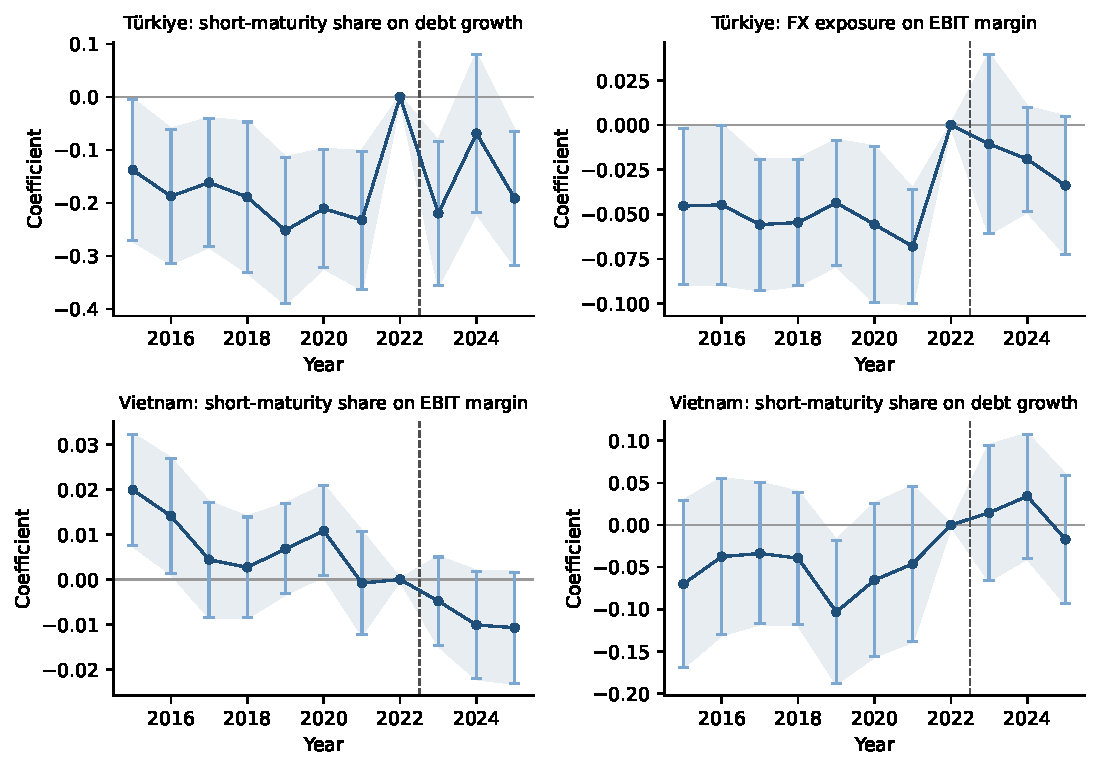
\includegraphics[width=\textwidth]{figs/event_studies.pdf}
\caption{Event studies of exposure interacted with year, with firm and year
effects and 95\% confidence intervals clustered by firm. The dashed line marks
the treatment date. Coefficients are non-zero well before treatment and do not
shift at it.}
\label{fig:events}
\end{figure}

Figure~\ref{fig:events} makes the point visually. Firms with more short-term
debt grow debt more slowly in every year from 2015
onward, and the coefficient at treatment is statistically indistinguishable from
those seven years earlier. The Vietnamese EBIT-margin result has the same
character, drifting from $+0.020$ ($p<0.01$) in 2015 to $-0.011$ ($p<0.10$) in
2025 and passing smoothly through the treatment year. These are persistent
differences between firm types, not responses to monetary policy. What a
conventional two-year window would report is the difference between the 2022
base and the 2023--25 average---a difference that exists, is significant, and
means nothing causal.

\section{Robustness}
\label{sec:robust}

\paragraph{Placebo treatment.} Assigning a false treatment at 2018 and
restricting to 2015--2021 returns nothing for Vietnam: $-0.791$ ($p=0.19$) on
interest coverage and $+0.004$ ($p=0.51$) on EBIT margin. The design is not
mechanically generating significance, which supports reading
Section~\ref{sec:results}'s significant coefficients as genuine pre-existing
trends.

\paragraph{Sample-size stability.} The Turkish estimates were computed at three
sample sizes as collection proceeded. At 83 firms the specification returned
$+0.886$ on the Altman $Z''$ score ($p=0.045$) with significant pre-trends; at
158 firms both vanished; at 585 firms the estimates are those of
Table~\ref{tab:main}. Roughly a third of the eventual sample produced a
significant wrong-signed result with apparent pre-trend violation.

\paragraph{Alternative specifications.} Results are unchanged under
winsorisation at 1\%/99\% rather than 2\%/98\%; exposure measured at 2020 or as
the 2020--21 mean; exclusion of the smallest asset tercile; and exclusion of
2022 to guard against restated comparatives.

\paragraph{What would overturn the null.} Table~\ref{tab:decomp} is explicit
that quarterly estimation would shrink $\sigma^2_u$, which was not the binding
constraint, and would leave $\sigma^2_\nu$ untouched. Portfolio sorting would
average away the transitory component at the cost of the heterogeneity that
motivates the exercise. Machine-readable disclosure of repricing basis would
remove the problem entirely.

\section{Implications for practice}
\label{sec:implications}

\emph{Validate the price measure against the policy path.} A measure that cannot
reproduce a known aggregate should not be used to estimate an unknown
cross-section; this test is what exposed the bundled-expense problem.

\emph{Report split-half reliability whenever exposure is estimated.} By
Proposition~\ref{prop:split} it is the attenuation factor itself, not merely a
diagnostic correlated with it, and by Proposition~\ref{prop:decomp} it separates
imprecision from impermanence. Standard errors and power calculations cannot:
in our data they indicated reliabilities of 0.78--0.99 where the true permanent
share was zero.

\emph{In inflation-accounting regimes, prefer flows.} By
Proposition~\ref{prop:restate} the contamination enters as an interaction and
fixed effects do not address it; by Proposition~\ref{prop:flow} ratios of flows
escape it.

\emph{Extend the pre-period until parallel trends can genuinely be tested.}
Restricting to outcomes with long history revealed that our significant
coefficients were decade-long trends; a two-year window would have produced a
publishable false positive.

\section{Conclusion}
\label{sec:conclusion}

Published financial statements support a genuine, validated measure of the price
of corporate debt, and it recovers monetary policy paths in a severe Turkish
tightening and a mild Vietnamese one. Using it we document pass-through of
roughly 35\%, a halving of median Turkish interest coverage, and a data field
that conflates currency shocks with interest costs.

Statements do not support a measure of which firms are contractually exposed to
repricing. Our framework explains why in a form that is testable rather than
rhetorical: the estimand is attenuated by the reliability of the exposure
proxy, that reliability is identified by a split-half correlation which is zero
in both countries, and the dispersion in estimated sensitivities is transitory
rather than permanent---so the failure is impermanence, which more data cannot
cure.

The implication is not that the channel fails to operate; our aggregate evidence
is consistent with its operating forcefully in T\"{u}rkiye. It is that the
cross-sectional question---\emph{which} firms bear the adjustment---requires
contractual data. Researchers without registry access should direct effort
toward the aggregate and price-side questions statements can answer, and toward
making repricing terms disclosable, rather than toward proxies that cannot carry
the weight placed on them.

\bibliographystyle{elsarticle-harv}
\bibliography{refs}

\end{document}
